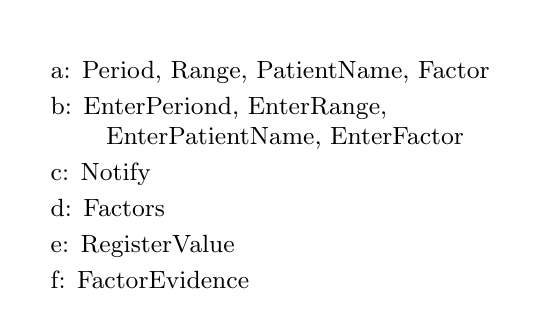
\begin{tikzpicture}
	%\draw[help lines,step=1cm,gray] (-2,-3) grid (12,3);

	\domain[x=0,y=0,type=machine]{m}{Monitor machine};
	\domain[x=0,y=2,type=designedDomain]{pr}{Periods \& Ranges};

	\domain[x=0,y=-2]{ms}{Medical staff};
	\domain[x=4.5,y=2]{ns}{Nurses' station};
	\domain[x=4.5,y=0]{fd}{Factors database};
	\domain[x=4.5,y=-2]{ad}{Analog devices};
	\domain[x=9,y=-2]{icu}{ICU patients};

	\connects[label position=left]{m}{pr}{a}
	\connects[label position=left]{m}{ms}{b}
	\connects{m}{ns}{c}
	\connects{m}{fd}{d}
	\connects[label position=below]{m}{ad}{e}
	\connects{ad}{icu}{f}


	\begin{scope}[align=flush left, text width=60mm, font=\small]
		\node at (9,1) {
		\begin{description}
		\itemsep0em
		\item a: Period, Range, PatientName, Factor
		\item b: EnterPeriond, EnterRange, EnterPatientName, EnterFactor
		\item c: Notify
		\item d: Factors
		\item e: RegisterValue
		\item f: FactorEvidence
		\end{description}
		};
	\end{scope}
\end{tikzpicture}

